\chapter{Complexity of Multicast Recycling Problem}

\section{NP-hardness Proof for Multicast Recycling}
\label{sec:mc-npc}

In this section, we first define a simplified version of \mcs, \mcos, that considers a \emph{single} primary tree and its backup tree for a given link.  Then, we prove \mco is NP-hard and use
this result to bound \mcs's complexity. To enhance readability, we drop the subscript from $T^l_i$, $\hat{T}^l_i$, $SA_i$, and $C_i^l$ when defining \mcos.
%The \mco formulation will prove useful in our coming complexity analysis. We define the decision problem for \mco below % because we study its NP-Completeness in this report.
%with some abuse of notation: we drop the subscript from $T^l_i$, $\hat{T}^l_i$, and $C_i^l$ to enhance readability. 

The \mco decision problem is defined as follows: %\textsc{Decision Problem}
\begin{itemize}

	\item  \underline{Instance}: $(G,k,T^l,l,\alpha)$.  $G=(V,E)$ is a directed, connected graph. $k$ is an integer greater than $0$ and $\alpha \geq 1$.
	$T^l=(V^l,E^l,r,D)$ is a primary tree containing nodes $V^l$, edges $E^l$ such that $l \in E^l$, has root $r$, and spans $D=\{d_1,d_2, ..., d_m\}$.
	%and is computed using the directed Steiner tree approximation algorithm specified in \cite{Charikar98}.

	\item \underline{Question}: Is there backup tree $\hat{T}^l=(\hat{V}^l,\hat{E}^l,r,D)$ such that $l \notin \hat{E}^l$ and $C^l \leq k$ under the condition that
		$w(\hat{T}^l) \leq \alpha \cdot w(SA(G'))$ where $G'=(V',E')$ such that $E' = E - \{l\}$; $SA(G') = (V_{A},E_{A},r,D)$ is a Steiner arborescence with root $r$ and spans $D$;
		and $w(\hat{T}^l_i)$ is the sum of $\hat{T}^l_i$'s link weights?
	%$\hat{E}^l,\setminus E^l \leq k$? 
	
\end{itemize}
Intuitively, we prove that \mco is NP-hard by showing that in some cases an optimal solution to \mco requires a solution to \arbors, a problem known to be NP-hard.
%The \arbor decision problem is to determine if a Steiner arborescence of cost less than $q$, where $q$ is a non-zero integer, exists.

\begin{theorem}
\label{thm:mco-npc}
\mco is NP-hard.
\end{theorem}
\begin{proof}
We reduce from the \arbor problem to show \mco is NP-hard.  Let the input to \arbor be a directed graph $G=(V,E)$ with unit link weights of $1$, root node $r \in V$, and
a set of terminal nodes $S \subseteq V$. For integer $q>0$, \arbor determines if an arborescence exists such that the sum of its link weights is less than or equal to $q$.
%We assume that each edge has unit weight of $1$. 
%The question is if a tree, $T$, exists that is rooted at $r$, has edges directed away from $r$, spans $S$, and the total weight of $T$'s edges is less than or equal to $q$.   

%We perform our reduction as follows. 
We perform our reduction as follows. % setting the input to \mcos as $(G',k,T^l,l,\alpha)$ where $T^l=(V^l,E^l,r,D)$.
We keep $r$ as the root node and set the terminal nodes $D = S$. We make a copy of $G$, $G^+$, and add a new node, $i$, to $G^+$ with edges $(r,i)$ and 
for all $d_j \in D$, $(i,d_j)$.  We let $T^l$ be the tree rooted at $r$, formed by the addition of edges $(r,i)$ and for all $d_j \in D$, $(i,d_j)$. Finally, we set $l = (r,i)$, $k=q$, and
and $\alpha = 1$. Figure \ref{fig:min-control-reduction} shows an example of this reduction procedure.

With this construction in place, we move on to show that a Steiner arborescence rooted at $r$ that spans $S$ with cost less than or equal to $q$ exists if and only if a
backup tree $\hat{T}^l=(\hat{V}^l,\hat{E}^l,r,D)$ exists in $G^+$ such that $l \notin \hat{E}^l$ and $C^l \leq k$ under the condition that $w(\hat{T}^l) \leq \alpha \cdot w(SA(G^+))$
In the remainder of this proof, we refer to $SA(G^+)$ simply as $SA$.

$(\Rightarrow)$  Given a Steiner arborescence in $G$, $A$, rooted at $r$, spanning $S$, and with cost $q$, we set $\hat{T}^l = A$. By construction $\hat{T}^l$ has root $r$, 
spans $D$, does not use $l$, results in $C^l \leq k$, and trivially satisfies $w(\hat{T}^l) \leq \alpha \cdot w(SA)$.


$(\Leftarrow)$ In the other direction, suppose we have a solution to \mcos, a backup tree $\hat{T}^l=(\hat{V}^l,\hat{E}^l,r,D)$ in $G^+$ such that
$l \notin \hat{E}^l$, $C^l \leq k$, and $w(\hat{T}^l) \leq \alpha \cdot w(SA)$.
Since we have fixed $l$ to be $(r,i)$ and $G^+$ is constructed such 
that the only incoming edge to $i$ is $(r,i)$, $T^l$ must be the tree formed by the edges $(r,i)$ and $\forall_{d_j \in D} (i,d_j)$. %formed using edges $(r,i)$ and $(i,d_j)$ for each $d_j \in D$. 
%is only connected to $r$ and each node in $D$, we can infer that $T^l$ must be tree formed using edges $(s,i)$ and $(i,d_j)$ for each $d_j \in D$. 
Because $l \notin \hat{E}^l$, by construction, it must be the case that $\hat{T}^l$ is edge disjoint from $T^l$.  
Since we have assumed that $C^l \leq k$, it must be the case that $\hat{T}^l$ has at most $k=q$ edges.  Lastly, we know that all nodes and edges in $\hat{T}^l$ 
exists in $G$, meaning that $\hat{T}^l$ forms a Steiner arborescence in $G$ rooted at $r$, spanning $S$, and has cost $q$.  This concludes our proof.
\end{proof}

%proof issues: (1) are E^l and E'^l disjoint or should it be specified as the corresponding trees

\begin{figure*}
  \begin{center}
    \subfigure[Graph $G=(V,E)$ where $S = \{a,b,c,d,e\}$ and $r$ are shaded blue.]{\label{fig:min-control-reduction1}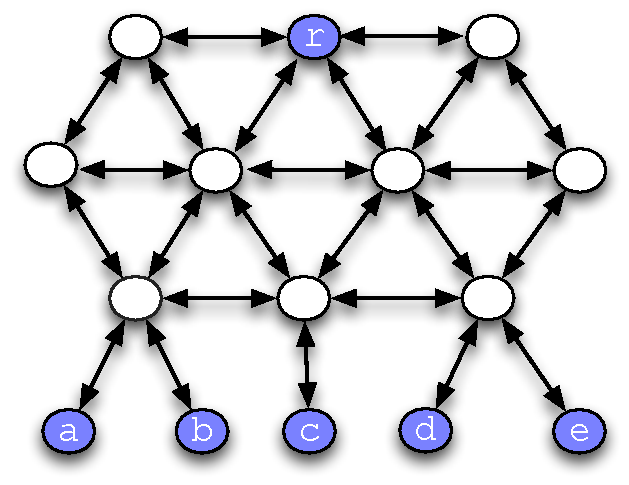
\includegraphics[scale=0.61]{figs/min-control-reduction1.pdf}}
    \subfigure[Graph $G^+=(V^+,E^+)$ resulting from our reduction in Theorem \ref{thm:mc-npc}.  
	All nodes ($i$) and edges ($i$'s incoming and outgoing edges) added $G$ by our reduction are dashed. The same dashed edges make up the primary tree in $G^+$, $T^l$.]
	{\label{fig:min-control-reduction2}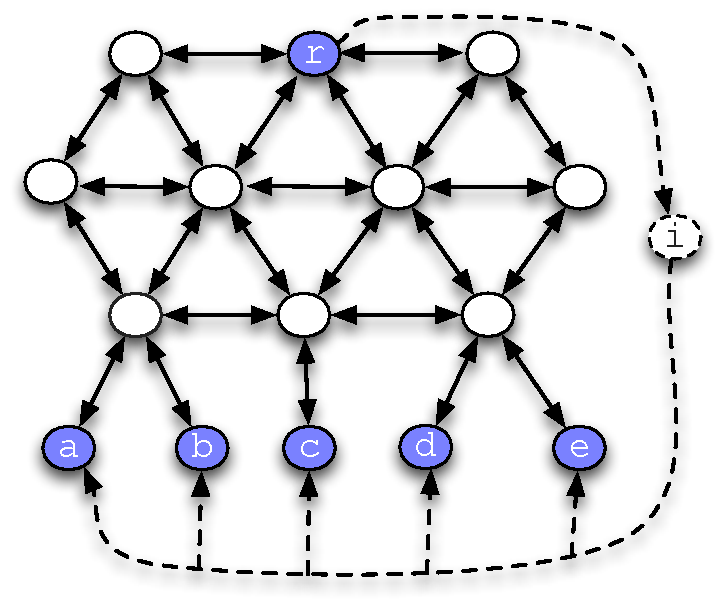
\includegraphics[scale=0.61]{figs/min-control-reduction2.pdf}}
  \end{center}
\caption{Example of reduction used in Theorem \ref{thm:mc-npc}.}
\label{fig:min-control-reduction}
\end{figure*}

\begin{theorem}
\label{thm:mc-npc-appendix}
\mc is at least NP-hard.
\end{theorem}
\begin{proof}
\mco is a special case of \mcs.  Since we have shown \mco is NP-hard in Theorem \ref{thm:mco-npc}, \mc must at least be NP-hard.
\end{proof}

